\section{DBSCAN Clustering Visualizations}\label{annexe:dbscan_visualizations}

\subsection{DBSCAN with Alternative Parameterization}

\paragraph{DBSCAN Clusters (PCA)}
A reduced number of clusters is obtained, with the majority of samples assigned to a single dominant cluster and only a minimal proportion labeled as noise.

\paragraph{Cluster Size Distribution}
One cluster overwhelmingly dominates the distribution, indicating a loss of density discrimination under this parameter configuration.

\paragraph{Fire Rate per Cluster}
Fire rates vary across clusters; however, the dominant cluster closely reflects the global fire rate due to its size.

\paragraph{Contingency Table}
Fire events are largely concentrated within the dominant cluster, limiting the discriminative capacity of the clustering.

\paragraph{Silhouette Analysis}
The average Silhouette score remains negative, confirming weak separation and internal inconsistency among clusters.

\paragraph{DBSCAN Summary}
This configuration reduces noise but collapses the clustering structure into a single dominant cluster, resulting in limited analytical value.

\begin{figure}[H]
    \centering
    
\includegraphics[width=0.8\linewidth]{images/DBscan/dbscan_from_scratch_analysis.png}
    \caption{Analysis of DBSCAN clustering implemented from scratch.}
    \label{fig:dbscan_from_scratch_analysis}
\end{figure}

\subsection{DBSCAN vs. Ground Truth (PCA Projection, Scikit-Learn) and (PCA Projection, From-Scratch)}

\paragraph{DBSCAN Clusters (PCA)}
DBSCAN identifies a limited number of dense regions primarily along the first principal component, while labeling a large proportion of samples as noise. Cluster boundaries do not align clearly with the global data structure.

\paragraph{Ground Truth Labels (PCA)}
Ground truth fire labels are widely dispersed across the PCA space with no clear linear separability, indicating a complex and overlapping class structure.

\paragraph{DBSCAN Clusters (PCA)}
The from-scratch implementation yields a similar cluster geometry, characterized by a strong dominance of noise points and limited cluster cohesion.

\paragraph{Ground Truth Labels (PCA)}
Fire and non-fire samples remain interwoven across the feature space, confirming the absence of clear density-based separation.

\begin{figure}[H]
    \centering
    
\includegraphics[width=0.8\linewidth]{images/DBscan/dbscan_pca_ground_truth.png}
    \caption{DBSCAN clustering results after PCA, compared to ground truth.}
    \label{fig:dbscan_pca_ground_truth}
\end{figure}

\begin{figure}[H]
    \centering
    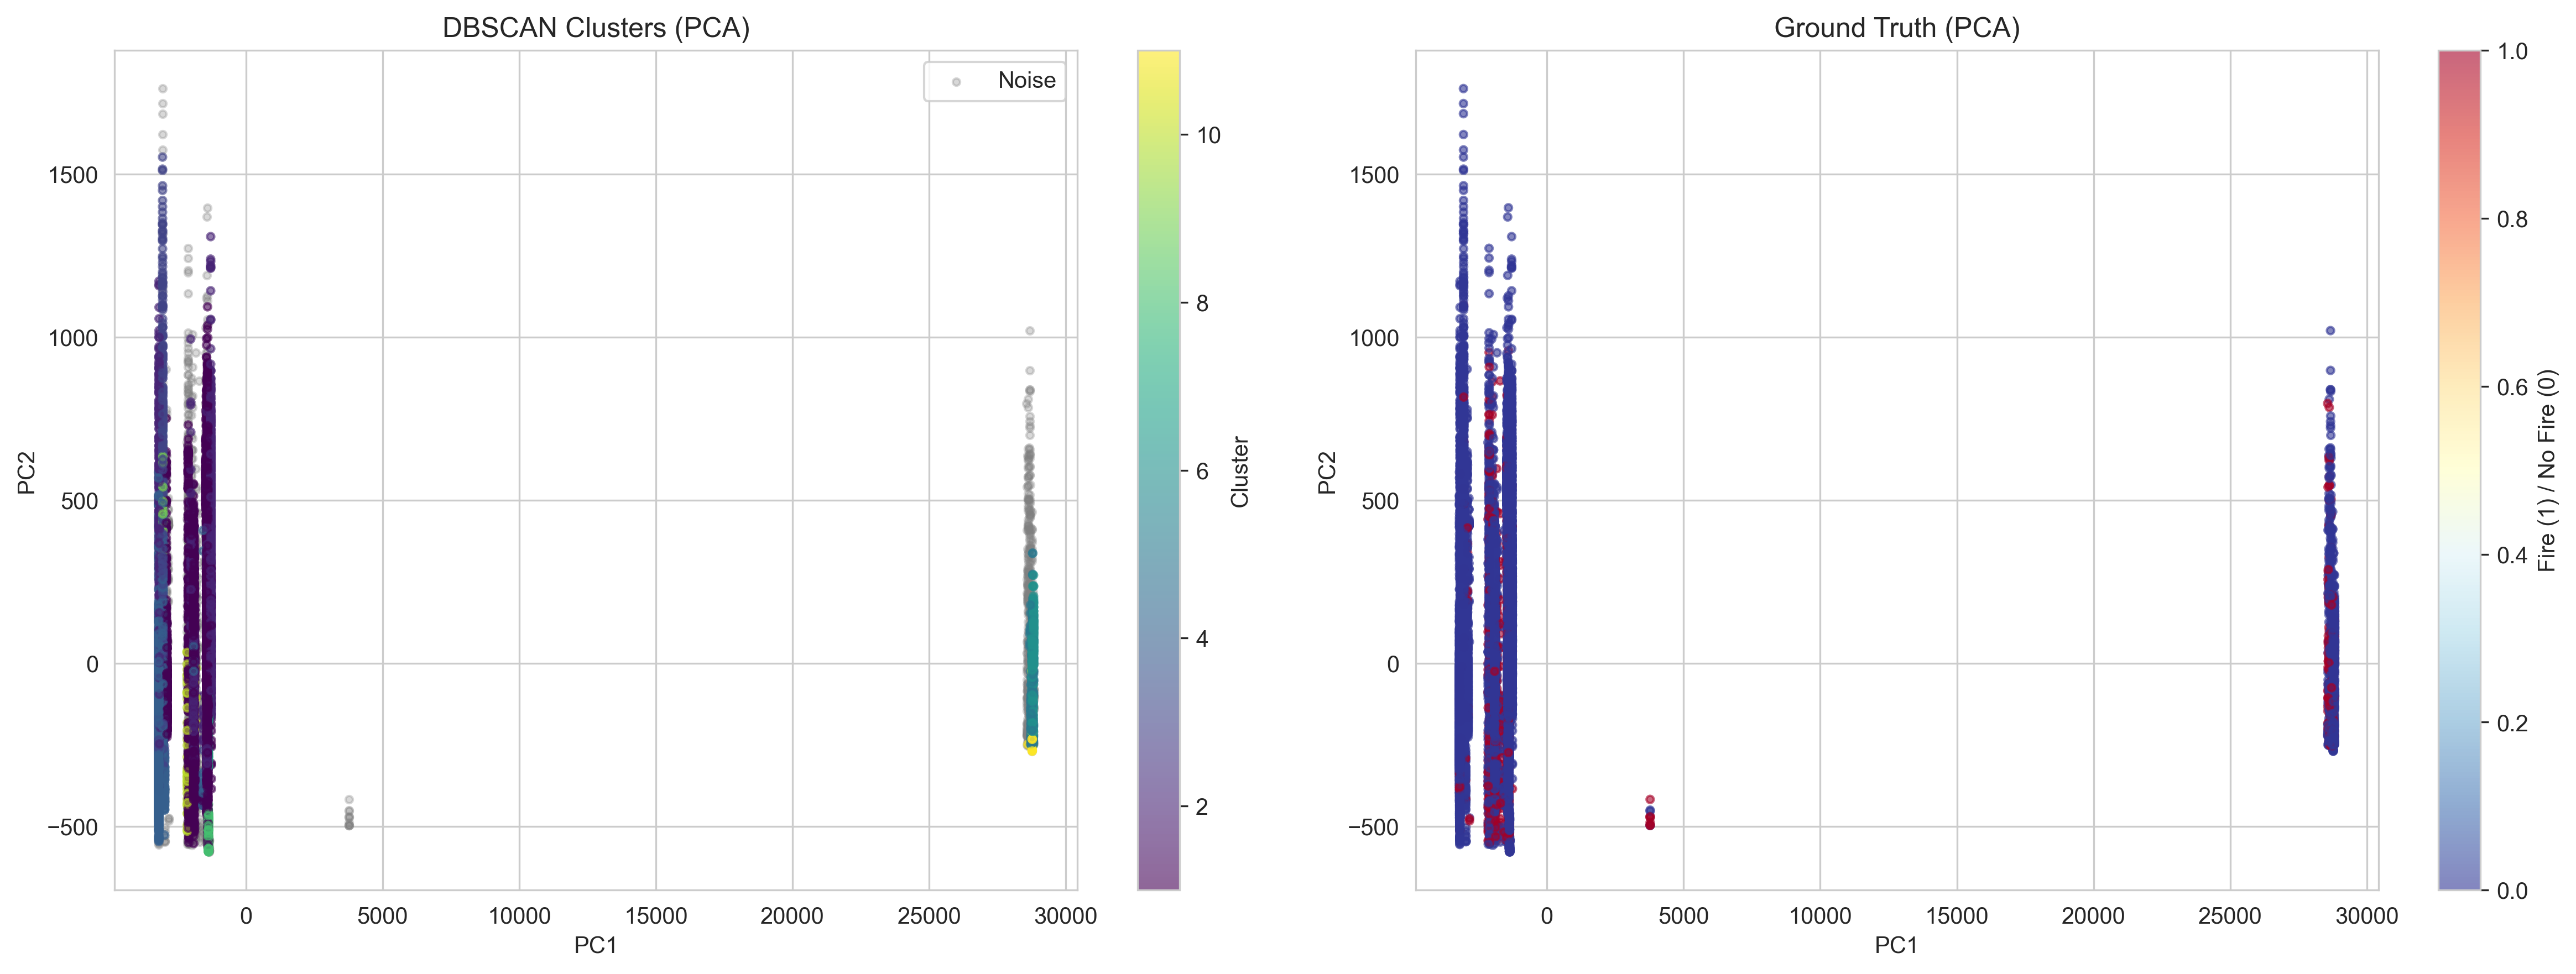
\includegraphics[width=0.8\linewidth]{images/DBscan/dbscan_pca_ground_truth_from_scratch.png}
    \caption{DBSCAN clustering from scratch after PCA, compared to ground truth.}
    \label{fig:dbscan_pca_ground_truth_from_scratch}
\end{figure}

\subsection{DBSCAN Detailed Analysis (Optimized Configuration)}

\paragraph{DBSCAN Clusters (PCA Projection)}
The clustering reveals multiple small clusters along with a non-negligible proportion of noise points. Cluster separation is primarily driven by the first principal component.

\paragraph{Cluster Size Distribution}
Cluster sizes are highly imbalanced, with a small number of dominant clusters and several very small ones, indicating heterogeneous density regions within the data.

\paragraph{Fire Rate per Cluster}
Fire occurrence varies significantly across clusters. Some clusters exhibit fire rates well above the global average, highlighting heterogeneous risk distributions.

\paragraph{Contingency Table (Fire vs. No Fire)}
The majority of samples correspond to non-fire instances across all clusters. Fire events are unevenly distributed, with certain clusters capturing a disproportionately higher number of fire cases.

\paragraph{Silhouette Analysis}
The average Silhouette score is negative, indicating substantial overlap between clusters and weak overall separation.

\paragraph{DBSCAN Summary}
Although the runtime remains acceptable, clustering quality is limited, as evidenced by negative Silhouette values and low agreement metrics.

\begin{figure}[H]
    \centering
    
\includegraphics[width=0.8\linewidth]{images/DBscan/dbscan_sklearn_analysis.png}
    \caption{Analysis of DBSCAN clustering using scikit-learn implementation.}
    \label{fig:dbscan_sklearn_analysis}
\end{figure}

\subsection{Bayesian Optimization and Optimized DBSCAN}

\paragraph{Bayesian Optimization Convergence}
The Silhouette score increases across iterations and stabilizes near its maximum value, indicating effective exploration and convergence of the Bayesian optimization process.

\paragraph{Parameter Space Exploration ($\varepsilon$, min\_samples)}
Higher Silhouette scores are observed for specific combinations of moderate $\varepsilon$ values and higher \texttt{min\_samples}. The selected configuration corresponds to a local optimum in the parameter space.

\paragraph{Optimized DBSCAN Clustering (PCA Projection)}
Clusters are mainly separated along the first principal component, which explains most of the variance. Several small clusters and noise points are detected, reflecting the sensitivity of DBSCAN to local density variations.

\paragraph{Metrics Comparison (Default vs. Optimized)}
The optimized configuration improves the Silhouette score and reduces the Davies--Bouldin index. The Calinski--Harabasz index decreases, which is expected given DBSCAN’s non-globular clustering structure and the presence of noise.

\begin{figure}[H]
    \centering
    
\includegraphics[width=0.8\linewidth]{images/DBscan/dbscan_bayesian_optimization.png}
    \caption{Bayesian optimization applied to DBSCAN hyperparameters.}
    \label{fig:dbscan_bayesian_optimization}
\end{figure}


\subsection{Overall DBSCAN Conclusion}
Although Bayesian optimization improves certain internal metrics, DBSCAN fails to produce well-separated and stable clusters for this dataset. The effectively one-dimensional data structure and overlapping class distributions substantially limit the effectiveness of density-based clustering methods.
